% Thesis introduction
% Author: Tore.
%

In this chapter the background information needed in order to understand the topics of this thesis and its papers is given. First, in Section \ref{sec:gpgpu} an introduction to general purpose programming on graphics processing units (\nom{GPGPU}{General purpose programming on graphics processing units}) is presented. Next, an introduction to ultrasound imaging is given in Section \ref{sec:ultrasound}.

\section{General-purpose computing on graphics processing units}\label{sec:gpgpu}

Architecture. See Paper II.

About theoretical FLOPS: Note that these are theoretical numbers and the actual throughput typically is algorithm dependent.

Add sentence about siemens and supersonic imagine scanners. They use GPUs? What does this mean? FPGAs and ASICs.

\begin{figure}
\centering
\includegraphics[width=0.9\textwidth]{img/free_lunsh.png}
\caption{Illustration of several transitions currently taking place in the computer industry. \todo{Site Herb Sutter - Welcom to the jungle http://herbsutter.com/welcome-to-the-jungle/}}
\label{fig:jungle}
\end{figure}

\begin{figure}
\centering
\subfigure[Threads, blocks and grid]{
	\includegraphics[width=0.4\textwidth]{img/cuda_threads.png}
}
\subfigure[Kernel]{
	\includegraphics[width=0.5\textwidth]{img/kernel.pdf}
}
\caption{Depicts how GPU threads are grouped into blocks and arranged in a grid. One thread runs a copy of a kernel function, in this example an element-wise matrix square operation.}
\label{fig:gpu_grid}
\end{figure}

\section {Ultrasound imaging}\label{sec:ultrasound}
Ultrasound imaging encompasses technology which generates images based on sound whose frequencies we can not hear. For medical ultrasound imaging frequencies above 2 MHz are typically used.

Small section about heart anatomy.

\begin{figure}
\centering
\subfigure{
	\includegraphics[width=0.47\textwidth]{img/Diagram_of_the_human_heart.png}
}
\subfigure{
	\includegraphics[width=0.47\textwidth]{img/HeartWall.png}
}
\caption{Overview of the human heart. Illustrations from wikipedia.org.}
\label{fig:human_heart}
\end{figure}

Typical probes, scan sequences, resolution and sampling.

Key selling points of ultrasound imaging: cost, safety and real-time user interaction.

One sentence about speckle tracking.
							
\subsection{Basic beamforming}

Delay and sum. Apodization. (See intro to Paper II or III).
Time v.s. phase delays.

\subsection{Adaptive Beamforming}\label{sec:adaptbf}

\begin{figure}[t!]
\subfigure[Delay-and-sum]{
	\includegraphics[width=0.47\textwidth]{img/scenario_das_resp2.png}
}
\subfigure[Capon]{
	\includegraphics[width=0.47\textwidth]{img/scenario_mv_resp2.png}
}
\caption{Array beam pattern with uniform and Capon weights. An interfering source is located at 20 degrees.}
\end{figure}

Capon beamforming\footnote{The name ''Capon beamformer'' is due to work by J. Capon \todo{add citation} on seismic arrays \todo{Move to background.}} or minimum variance beamforming.

Intro to adaptive beamforming. List other variants (LCA, beamspace, Eigen space etc.). 

Beamspace data is typically refers to the polar grid that cardiac ultrasound data is located in prior to scan conversion. In combination with the Capon beamformer, beamspace refers to the K-space representation of the impinging signals (hence the \nom{FFT}{Fast fourier transform} of the channel data). 

Not phase aberration correction.

Add section about the computationally complexity. How many flops are required per rx-beam etc...

Add section about how to present data (max v.s mean etc.)
						
\subsection{Shift invariance}

\section{Volume rendering}

Get section from master theses. Ray casting and opacity functions.

\begin{figure}
\centering
\subfigure[Ray-casting]{
	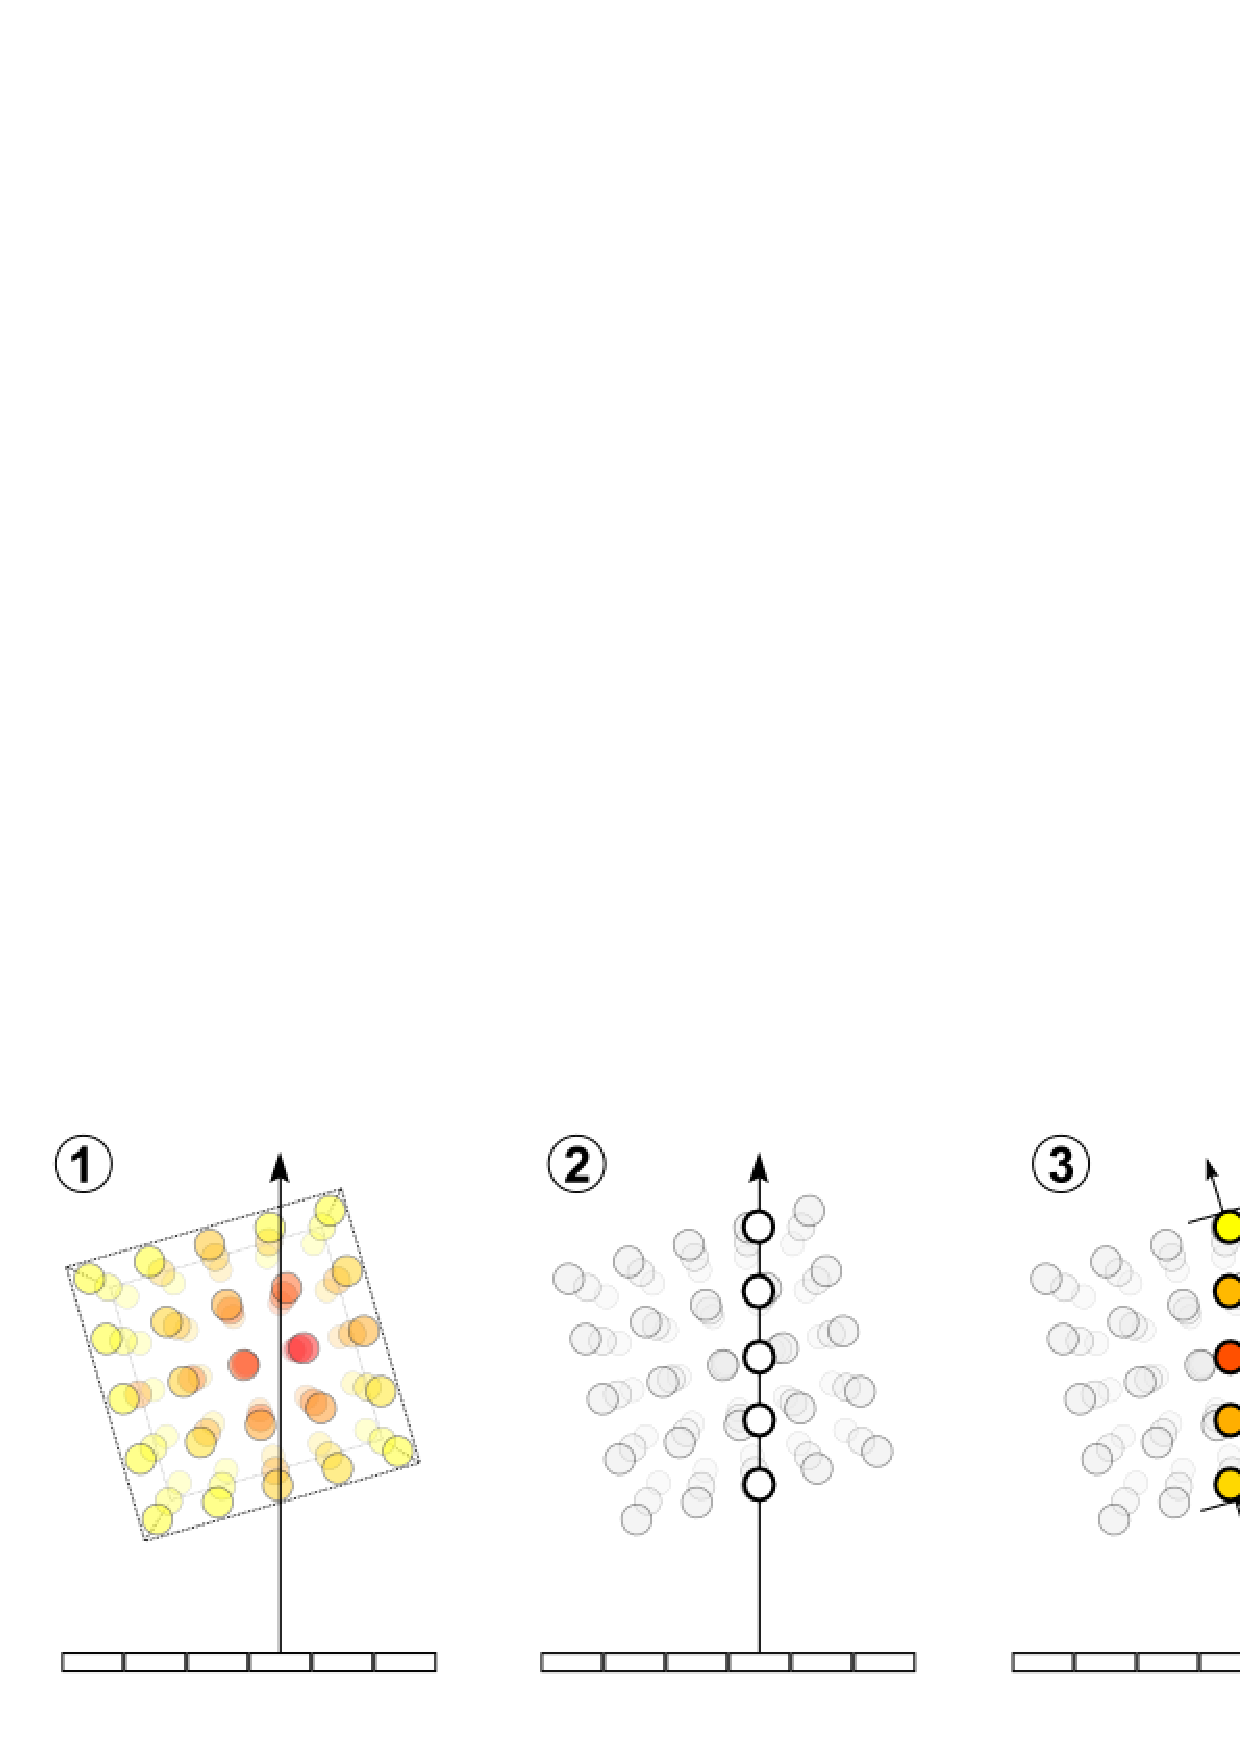
\includegraphics[width=0.4\textwidth]{img/Volumeraycasting.png}
}
\subfigure[Opacity transfer function]{
	\includegraphics[width=0.5\textwidth]{img/otf.png}
}
\caption{.}
\label{fig:vr}
\end{figure}

\subsection{Adaptive volume rendering}

Visibility driven visualization.

\section{Field simulations}

Small chapter about different simulation tools (See hos paper).
			
\endinput
